\documentclass[twoside,twocolumn]{article}

\usepackage{blindtext} 
\usepackage[T1]{fontenc} 
\usepackage[english]{babel}
\usepackage[hmarginratio=1:1,top=20mm,columnsep=20pt]{geometry}
\usepackage[hang, small,labelfont=bf,up,textfont=it,up]{caption}
\usepackage{booktabs}
\usepackage{array,graphicx}
\usepackage{pifont}
\usepackage{amsfonts}
\usepackage{float}
\usepackage{natbib}
\usepackage{amsmath,amsthm}
\usepackage{enumitem}
\usepackage{relsize}
\usepackage{algorithm}
\usepackage{bm}
\usepackage{algcompatible}
\usepackage{caption}
\captionsetup{skip=0pt}
\setlist[itemize]{noitemsep}
\usepackage{titlesec} 
\titleformat{\section}[block]{\large\scshape\centering}{\thesection.}{0.5em}{} 
\titleformat{\subsection}[block]{\scshape\centering}{}{0.5em}{} 
\usepackage{titling} 
\usepackage{hyperref}
\setlength{\droptitle}{-4\baselineskip}
\pretitle{\begin{center}\Huge\bfseries}
\DeclareMathOperator*{\argmin}{arg\,min}
\posttitle{\end{center}}



\setlength{\intextsep}{5pt plus 2pt minus 2pt}
\titlespacing*{\section}
{0pt}{1.0ex plus 1ex minus .2ex}{2.0ex plus .2ex}
\titlespacing*{\subsection}
{0pt}{1.1ex plus 1ex minus .2ex}{1.5ex plus .2ex}
\font\myfont=cmr12 at 18pt
\title{\myfont Sentiment Classification of Movie Reviews on IMDB} % Article title
\author{
\textsc{Gabriele Dragotto$^a$, Jiaqi Liang$^a$, Kaiqiong Zhao$^b$}\\[1ex]
\normalsize $^a$CERC Data Science for Real-Time Decision-Making, Polytechnique Montreal.\\ 
\normalsize \{gabriele.dragotto,jiaqi.liang\}@polymtl.ca\\ 
\normalsize $^b$McGill University \\ 
\normalsize kaiqiong.zhao@mail.mcgill.ca
}
\date{COMP551 (Winter 2019) - Project 2}
\renewcommand{\maketitlehookd}{







\begin{abstract}
\noindent The IMDB sentiment classification is a popular benchmark for classification models \citep{maas2011learning}. In this project, we introduce and compare several textual, both from literature and with out experimentation. We test and benchmark different classifiers with extensive cross-validation and hyper-parameter search. In the first instance, we design a 3 feature model based on common words occurences, POS words, and n-grams. , Naive Bayes, logistic regression, SVM, and Decision tree classify the training set with a 5-fold CV and randomized hyperparameter tuning. Finally, an exhaustive hyperparameter-search is performed to select the best performing classifier, which predicts the test-set for the Kaggle competition. According to out methodology, an SVM with lemmatization and word-preprocessing provides the best accuracy (90.8\%) over the provided test-set.
\end{abstract}
}
\begin{document}
\maketitle


\section{Introduction}
Sentiment classification is a special subfield of text classification, and focuses on automatic text classification into polarity levels (eg, positive and negative). The vast amount of data available from online social communities booss the interest from the machine learning community, mostly for supervised and semi-supervised learning applications.
In particular, the IMDB sentiment classification task is a popular benchmark \citep{maas2011learning} for natural-language based classification methodologies. In this project, we develop an accurate sentiment classification model for the IMDB datased, in order to classify movie reviews as positive or negative. 
In particular, we start with a standard feature selection - namely common words occurrences, part-of-speech (POS) and 2-grams - and evolve our models on top of it. We consider many combinations of features and preprocessing techniques, such binary occurrences of popular words or their idf transformed. Several classifiers produces predictions with a 5-fold cross-validation on the training-set. In particular, we compare Logistic regression, Decision tree (DT), naive Bayes (NB), and support vector machines (SVM). An exhaustive search for classificatiors' hyperparameter and pre-processing techniques provides the best-performing recipe for our task. We present a benchmark of compared results for the introduced classifiers and parameters.


\subsection{Related work}
Sentiment classification plays an important role in the effort to better organize the vast amount of data we produce each day. The task attracts the interest of both the linguists and machine-learning community \citep{pang2002thumbs}. In particular, a recent work by \cite{Medhat2014ensemble} discerns between lexicon-based and machine-learning approaches. In the latter, the classification leverages on the creation of text-based features, for instance bag of words (BoW), and word-vector representations \citep{mikolov2013exploiting}. These features incorporates with different classifiers like NB, SVM, and DT, and produce reasonably accurate results \citep{pang2002thumbs}. On the other side, BoW neglects information such as word order in the sentence, word relations, and hidden semantic structures, eventually reducing the effectiveness of sentiment analysis. Thus, POS and n-gram are usually complementing models to improve their accuracy. \citep{al2017automatic} reports positive results on ensamble methods, hence combining several classifiers to enhance performances. Other works (\cite{Cata2017ensemble}, \cite{Chalothom2015ensemble}) investigats the effectiveness of ensamble methods. \cite{xia2011ensemble} surveys different feature selections with different classifiers, and states syntactic relations plays a significant role sentiment classification. 
Hyperparameter settings can also induce significant performance gaps between models. \citep{bergstra2012random} provides a positive result for randomized hyperparameter search compared to exhaustive search.



\section{Dataset}
\label{sec:dataset}
The dataset contains $25000$ reviews from the IMDb database. The training-set is equilibrated, with $12500$ positive reviews and $12500$ negative ones. We employ several text pre-processing techniques to prepare the data.
\begin{itemize}
    \item \ Tokenization: the text is split into words, and stopwords, numbers, and special characters (eg, HTML tags) are removed.
    \item \ Lemmatization: words trace back to a basic inflected form.
    \item \ Common words extraction: return the most $k$ frequent words in the training set.
    \item \ POS words extraction: extracts the most k frequent adjectives, adverbs, verbs, and nouns.
    \item \ n-gram: extracts subsets of n consecutive words from the text.
\end{itemize}

	
\subsection{Setup}
\label{sub:setup}
A 5-fold cross validation scheme evaluates prediction accuracies for different feature selections (see Section \ref{feature}), and different classification models (Section \ref{class}).
An exhaustive grid-search for hyperparameters and text-processing returns the best performing settings.
\section{Proposed approach}
\subsection{Feature design} \label{feature}
Our methodology is based on 3 sets of features, namely common words, part-of-speech (POS), and n-grams. For each subset, we implement either the binary feature (eg, the word occurs or not) or the idf transformation (see Table \ref{tab1}).

\begin{itemize}
	\item \textit{commonWord}: $cword\_O_{k}$, $cword\_T_{k}$, $cword\_OS_{k}$, $cword\_TS_{k}$.
	\item \textit{posWords}: $POS\_O_{k}$,$POS\_T_{k}$.
	\item \textit{n-gram}: $gram(1,2)\_O_{k}$, $gram(1,2)\_T_{k}$, $gram(2,2)\_O_{k}$,$gram(2,2)\_T_{k}$, $gram(2,3)\_O_{k}$,$gram(2,3)\_T_{k}$.
\end{itemize}
With $k$ we model the number of most frequent words. $cword\_O_k$ models the binary occurrence of the $k-th$ most frequent word, while $cword\_T_k$ is the TF-transformed occurrence of it. $cword\_OS_k$ and $cword\_TS_k$ represents the same statistics with lemmatization. In terms of n-grams, $gram(a,b)$ represents the set of $n-grams$ with length from $a$ to $b$.




\section{Classification Algorithms}
\label{class}

\subsubsection{Bernoulli Naive Bayes}
We model a Bernoulli Naive Bayes classifier to predict sentiment status using the common-word-based binary occurrence features. Let $Y$ be the binary random variable indicating whether a movie comment is positive, and $x_i$ the occurrence indicator of word $i$, for $i = 1, 2, \ldots, k$. Let $\boldsymbol{X} = \left(x_1, x_2, \ldots x_k \right)$ be the binary feature vector. With Bernoulli Naive Bayes assumptions, $x_i$ are mutually independent from each other. The conditional probability of observing feature $\boldsymbol{X}$ in class $Y=j$, where $j = 0, 1$, is in Equation (\ref{eq:nb}).
\begin{equation}
\begin{split}
P(\boldsymbol{X}|Y=j)=\\ \prod_{i=1}^{k} \left[P(x_{i}|Y=j)\right]^{x_i}\left[1-P(x_{i}|Y=j)\right]^{1-x_i} \;  \\
j \in \{0, 1\} 
\label{eq:nb}
\end{split}
\end{equation}

%In the given dataset, we have the prior probabilities $P(Y=0) =P(Y=1) = 1/2$. 
In addition, the probability of observing a given feature $\boldsymbol{X}$ coming from class $j$ can be calculated as $P(Y=j|\boldsymbol{X}) \propto P(Y=j) P(\boldsymbol{X}|Y=j) $. The predicted class is the $j-th$ one, namely the one with a greater value. The vocabulary injected for this hard-coded Bernoulli Naive Bayes is the top $k=450$ common words (i.e. $cword\_O_{450}$). This approach yields an average validation accuracy  $80\%$ over our training-set.

%Here we simply use the $cword\_O_{k}$ without stopwords of the training set to train the model and get an approximate $80\%$ accuracy via cross validation when $k=450$.
\subsubsection{Multinomial Naive Bayes}
Multinomial Naive Bayes is slight modification of the Naive Bayes approach, dealing with features with non-integer values, such as the ones derived from TF-IDF \citep{kibriya2004multinomial}.
We applied the Multinomial Naive Bayes classifier on the TF-IDF feature set, where the vocabulary is extracted following the three different definitions outlined in Section \ref{sub:setup}.
%word counts or fractional counts 
%In the multinomial Naive Bayes, a text is represented by an ordered sequence of multinomial distribution words via term frequency.  
\subsubsection{Logistic Regression}
Logistic regression is a discriminative classification approach capturing the posterior probability of a target variable given the observed feature (i.e. $P(Y|\boldsymbol{X})$). It usually performs better when there is greater confidence in the correct specification of $P(Y|\boldsymbol{X})$ relative to $P(\boldsymbol{X}|Y)$ \citep{xue2008comment}. We explored the performance of logistic regressions under different combinations of the entire features, and with different $L2$ regularization parameters ($C$). 

 
\subsubsection{Decision Tree}
A decision tree classifier is a hierarchical model consisting of a set of decision rules which recursively split input features into homogeneous zones  \citep{breiman2017classification}. It can automatically handle input features showing highly nonlinear relationships, and results can be easily interpreted.  
%Decision tree has been applied successfully in many classification situations
%Decision tree is a method for approximating discrete-valued target functions, in which each internal node represents a test on an attribute and each leaf node reveals a class.
Decision tree has a simple structure and relative high efficiency in specific classification tasks \citep{murthy1998automatic, apte2001method}. In our experiments,  trees trains with different maximum depths, under different combinations of features. In general, their accuracy on the training-set is lower than other models (less than 80\%).

\subsubsection{Support Vector Machine}
SVM is a discriminative classification method learning, one of the so-called decision boundary methods. It create an optimal hyperplane maximising the distance between classes in the multidimensional feature space \citep{vapnik2013nature}. It can handle non-linearly separable data by applying an appropriate kernel to mapping the original input space into a high-dimensional feature space \citep{smola2004tutorial}. 
We first trained our SVM model on a feature space of individual and bigram words (approx 1,522,587 features), with different regularization parameters $C$ (a grid from $0.01$ to $10$ with steps of $0.2$) and different types of kernels (linear, polynomial or Gaussian kernels). Overall, the linear SVM yields a higher validation accuracy compared to the others. 
Results of \cite{joachims1998text} shows that text classification problems can frequently be efficiently tackled well with linear SVM, due to the sparse and high dimensional nature of the features. Our results confirm such findings.
%and linear separability in most text classification tasks,
%linear kernel is commonly used. \cite{joachims1998text} % Citations? 
Hence, we focused on the linear SVM with different regularization parameters to investigate the best feature combinations yelding a better validation accuracy on the provided training-set.

%SVM is a another discriminative model, where the decision boundaries are learned by maximizing the margin.Both the feature combinations and the SVM parameters including penalty coefficient $C$ are considered in our experiments. 



\section{Results}
We combined  three feature sets with the common words vocabulary(set 1), the top Part-of-Speech words $k=2000$ (set 2), and the (1,2)-grams words (set 3). Respective weights are of $\eta_1, \eta_2$ and $\eta_3$. The results confirms that a relative large weight on the Bag of words-based features (n-gram), i.e. $\eta_3$ usually leads to a better average validation accuracy. 
In addition, the use of TF-IDF transformed counts improves the validation accuracy, compared to the scenarios where we only used the binary occurrence.
In the terms of different classifiers, the decision tree do not perform well in our experiments, and yields an accuracy below 80\%. The results for Logistic regression and Multinomial Naive Bayes do not surpass our best SVM benchmark.


\begin{figure}[h]
\centering
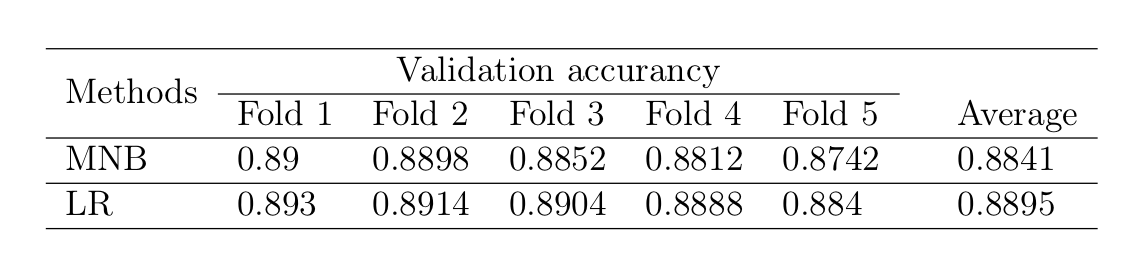
\includegraphics[width=0.5\textwidth]{Compare.png}
\caption{Validation accuracy for the best multinomial naive bayes and linear regression that we searched from the combination of 3 feature sets with weighted (1) $\eta_1 =1, \eta_2 = 0.2, \eta_3=1$ and (2) $\eta_1 =0.5, \eta_2 = 0.2, \eta_3=1$ and (3) $\eta_1 =0.2, \eta_2 = 0.2, \eta_3=1$. The regularization paramters $C$ was specified in a range between 0.1 and 8.5 with increment 0.5.}.
\label{fig:Fig1}
\end{figure}


\begin{table}[h]
\centering
\resizebox{0.5\textwidth}{!}{
\begin{tabular}{@{}lll@{}}
\toprule
\textbf{Hyperparam:} & C=7.25 & \textbf{} \\
\textbf{Mean-Acc-Score:} & 0.912 (0.002 std) &  \\ \midrule
\textbf{Set} & \textbf{Param} & \textbf{w} \\ \midrule
\textbf{CommonW} & IDF & 0.2 \\
\textbf{POS} & IDF & 0.85 \\
\textbf{n-grams} & \begin{tabular}[c]{@{}l@{}}n-gram(1,2)\\ Occurrence\\ IDF\end{tabular} & 2.1 \\ \bottomrule
\end{tabular}
}
\caption{ Best performing results for SVM classifier
\label{svm_res}}
\end{table}

\section{Discussion and Conclusion}
We provide a comprehensive study of various text features and base classification algorithms for sentiment classification. Based on a discrete set of empirical experiments, the pre processing of text played a fundamental role. Moreover, the BagOfWord (up to 2-grams) features effectively contributed to the classification task. The $SVM$ machine with an l2 regularization ($C=7.25$) yelds a $91.2\%$ accuracy on our 5-fold cross-validated training set. Extensive report on the best performing model is available in Table \ref{svm_res}.
We tested ensemble methods using either majority vote or weighting to combine the prediction from our base estimators in Section \ref{class}, but no significant improvement was achieved. This might be because the weighted sum of all the prediction is not dichotomous, and the additional dichotomization makes the optimization of the loss function intractable \cite{polley2010super}. An ensemble classifier with a more diverse set of base estimators and other aggregation techniques \citep{parvin2013classifier} can be worth exploring.   
In addition, our analysis treats the individual or n-gram words independently and their sequential nature in a speech is ignored. However, the word vector of the text is likely to improve the classification accuracy \citep{mikolov2013exploiting}. Moreover, other classifier like recursive neural network (RNN) or deep learning models, accounting for the word embedding structures, can constitute viable options. 

\section*{Statement of Contributions}
\begin{enumerate}[topsep=2pt,itemsep=0ex,partopsep=1ex,parsep=1ex]

	\item Gabriele [33\%]: implementation, testing and submission. Latex writing and proofreading
	\item Jiaqi [33\%]: implementation, testing. Writing and results.
	\item kaiqiong [33\%]: implementation, testing and submissions. Results and writing

\end{enumerate}



\renewcommand*{\bibfont}{\footnotesize}



\bibliographystyle{elsarticle-harv}
\bibliography{Biblio.bib}



\end{document}
